% Just The Docs Front Matter
% title: Uncertainty Quantification (UQ)
% parent: Tutorials
% has_children: false
% has_toc: false

\subsection{Uncertainty Quantification (UQ)} \label{sec:using-issm-tutorials-uncertaintyquantification}
\subsubsection{Goals} %{{{
\begin{itemize}
	\item Use ISSM to assess how errors in model inputs propagate through a 2D SSA steady state ice flow model
	\item Use ISSM to assess how ice flow model diagnostics (e.g. velocity, mass flux, volume) can be affected by perturbations to input in other parts of the model domain
	\item Become familiar with the uncertainty quantification (Dakota-based) tools available in ISSM
\end{itemize}

Go to \lstinlinebg|<ISSM_DIR>/examples/UncertaintyQuantification/| to do this tutorial.

%}}}
\subsubsection{Introduction}%{{{
This experiment will use the model of Pine Island Glacier that was saved in the previous 
%__@LATEX_ONLY_START@__
\hyperref[sec:using-issm-tutorials-pig]{Pine Island Glacier modeling tutorial}.
%__@LATEX_ONLY_END@__
%__@MARKDOWN_ONLY_START@__
% <a href="pig">Pine Island Glacier modeling tutorial</a>.
%__@MARKDOWN_ONLY_END@__
It aims to use the ISSM-Dakota integrated model system to (1) quantify the uncertainties of model output in response to errors in model input and (2) quantify sensitivities of model output to spatial perturbations in model input.
\begin{itemize}
	\item Our model inputs: ice thickness, ice rigidity, and basal friction.
	\item Our model outputs: mass flux at 13 flux gates across PIG.
\end{itemize}
Our Uncertainty Quantification (UQ) methods are based on the Design Analysis Kit for Optimization and Terascale Applications (Dakota) software \citep{Eldred2008}, which is embedded in ISSM. The following diagram illustrates the relationship between ISSM and Dakota. The ISSM mesh must be partitioned (i.e. vertices can be grouped together so that Dakota varies them together - this is helpful when you want to vary equal areas over the unstructured mesh). To partition the mesh, you can do so linearly (one partition per vertex), or you can use an external package software like Chaco to weight vertices and create the partitions you desire. Dakota is responsible for varying the provided inputs in the user-defined way (uniform, normal, etc.) for each mesh partition and then launching an ISSM run with the perturbed forcing. Dakota is also responsible for creating statistics for output, which are also user defined. Output diagnostics include ice mass flux through defined gates and scalar output (e.g. Ice Volume, Total SMB, etc.).
\begin{figure}[H]
	\begin{center}
		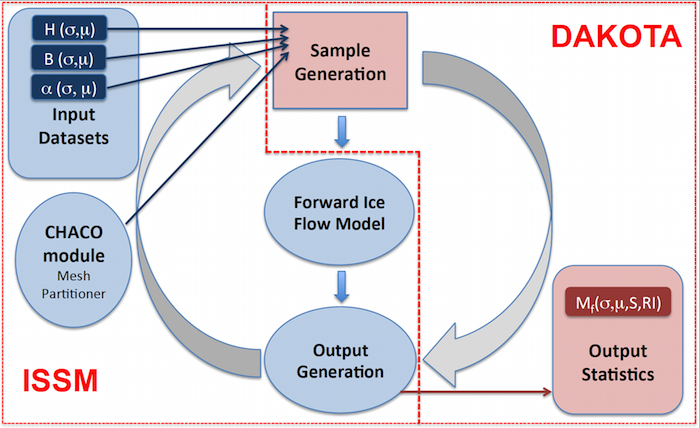
\includegraphics[width=\textwidth]{\assetsParentPath/assets/img/using-issm/tutorials/uncertaintyquantification/ISSMUQDiagram.png}
	\end{center}
\end{figure}

Tutorial steps to be taken:
\begin{itemize}
	\item Begin by loading results from the \lstinlinebg|examples/Pig| tutorial (the end of basal friction inversion)
	\item Load ice thickness cross-over errors from IceBridge 2009 WAIS campaign
	\item Run sampling analysis using ice thickness cross-over and mass flux diagnostics
	\item Run sensitivity analysis using ice thickness, ice rigidity, and basal friction as inputs and mass flux diagnostics
	\item Plot results: partition, sampling, and sensitivities
\end{itemize}
Sampling Analysis:
Quantify the uncertainties of model output (diagnostics like mass flux, Ice Volume, Max Velocity) in response to errors in model input. The figure below illustrates an example of Sampling errors in ice thickness. The result for each gate, is a histogram of Mass Flux (one value per each model run, or sample).
Below is the resulting histogram for mass flux gate 2.
\begin{figure}[H]
	\begin{center}
		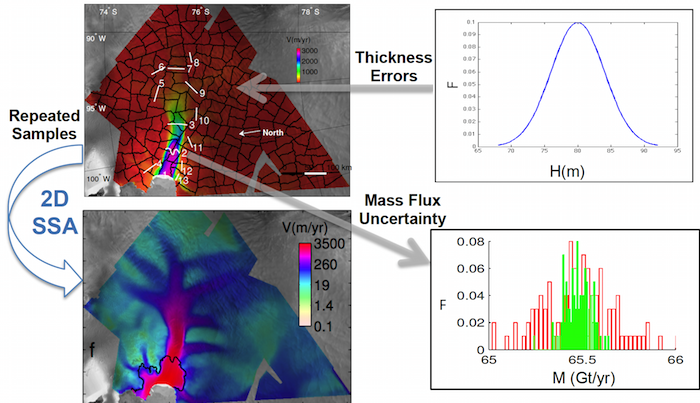
\includegraphics[width=\textwidth]{\assetsParentPath/assets/img/using-issm/tutorials/uncertaintyquantification/Sampling.png}
	\end{center}
\end{figure}

Sensitivity Analysis:
Quantify sensitivities of model output to small spatial perturbations in model input. The figure below illustrates how this is accomplished. One by one, partition input is changed by a small percentage, and a model run is launched. For this specific run, changes in model diagnostics (output) are assessed by Dakota. This is done for each partition, such that the number of model runs is equal to the number of mesh partitions. In the end, every diagnostic is associated with a sensitivity value at every partition. In this way, we can make a map of sensitivities for each diagnostic. Sensitivities can also be ranked, for each diagnostic, in importance. One such example of Dakota output is the `importance factor', or sensitivities scaled by error margins
\citep{Larour2012a, Larour2012b}, illustrated below as UQ sensitivity analysis output for mass flux
gate 2.
\begin{figure}[H]
	\begin{center}
		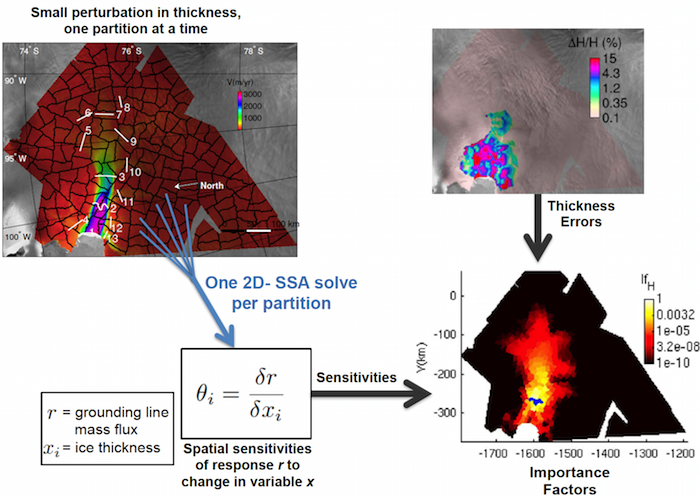
\includegraphics[scale=0.62]{\assetsParentPath/assets/img/using-issm/tutorials/uncertaintyquantification/Sensitivity.png}
	\end{center}
\end{figure}

For manuscript examples of these studies, see
\cite{Larour2012a,Larour2012b,Schlegel2013,Schlegel2015}.

%}}}
\subsubsection{Flux Gates} %{{{
Flux gates are ARGUS (\lstinlinebg|*.exp|) files found in \lstinlinebg|./MassFluxes|. The gates are positioned across PIG at the inset of tributary glaciers.

Mass fluxes will be computed in (Gt/yr) for all of these gates (using the depth-average ice velocity, ice thickness, and ice density).

Run step 1 of the \lstinlinebg|runme.m| to plot the gates overlaid over the PIG surface velocities.
\begin{figure}[H]
	\begin{center}
		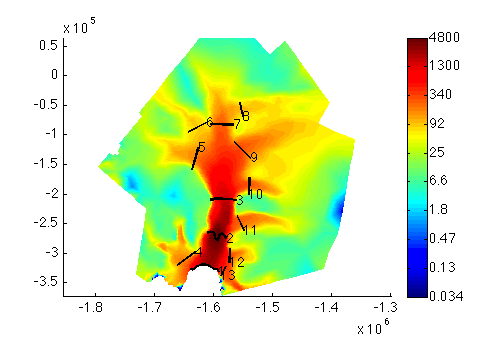
\includegraphics[width=\textwidth]{\assetsParentPath/assets/img/using-issm/tutorials/uncertaintyquantification/FluxGates.png}
	\end{center}
\end{figure}
%}}}
\subsubsection{Loading Cross-Over Errors} %{{{
For ice thickness errors we will use McCords cross-over errors from CReSIS. First you will load errors. Some of these errors are too large, too small, or need to be interpolated onto a larger domain (you will filter these out). Load cross overs \lstinlinebg|'../Data/CrossOvers2009.mat'|. Interpolate cross over errors over our mesh vertices. Avoid \lstinlinebg|NaN| values. Filter out unrealistic error ranges. Avoid large unrealistic values. Transform into absolute errors and setup a minimum error everywhere.

Run Step 2 in the \lstinlinebg|runme.m| to load the crossover errors.
%}}}
\subsubsection{Sampling Analysis} %{{{
In order to accomplish the sampling step, we must first partition the mesh into equal area partitions. We'll start with 50. You can try and play with the package for partitioning (`chaco' or `linear'), the number of partitions, and weighting (`on' or `off'):
\begin{itemize}
	\item See lines 69-72 in the \lstinlinebg|runme.m| file
	\item Run step 3
\end{itemize}
To plot the corresponding partition over a plot of the mesh:
\begin{itemize}
	\item See lines 155-162
	\item Run step 4
\end{itemize}
\begin{figure}[H]
	\begin{center}
		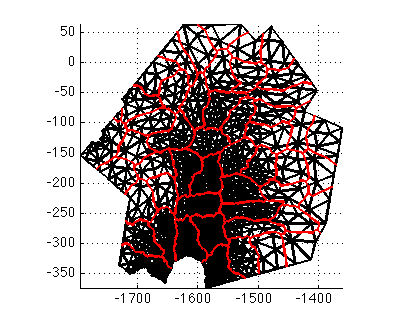
\includegraphics[width=\textwidth]{\assetsParentPath/assets/img/using-issm/tutorials/uncertaintyquantification/Partitions-1.png}
	\end{center}
\end{figure}
Note that after using Chaco, your partitions may look different from those illustrated here, because there is a randomness to the Chaco algorithm, and results differ on different computer systems.

Second, we must define our UQ input. Here, we will sample ice thickness (H), so we must define errors on each partition for H with a corresponding PDF (Probability Density Function). Here we calculate the crossover errors on each partition. In this example, we will sample a normal error distribution around every partition. To do so, we need to specify to Dakota that we want a normal sampling, and we must provide the standard deviation of error at every partition. Because crossover errors represent the full range of thickness errors, we assume this represents a 6-sigma normally distributed spread. Therefore, we set the standard deviation equal to the crossover error at a particular location, divided by 6:
\begin{itemize}
	\item See lines 74-82
\end{itemize}

Third, we must set up the desired diagnostics, or output responses. In this case, we choose ice mass flux at 13 flux gates around the domain:
\begin{itemize}
	\item See lines 84-97
\end{itemize}

For all responses, we specify a string identifier and the desired output confidence intervals. We also need to specify an \lstinlinebg|*.exp| file to define each flux gate, and directory where to find the latter:
\begin{itemize}
	\item See lines 99-115
\end{itemize}

Finally, we need to designate a sampling strategy. Options include \lstinlinebg|'nond_samp'| for sampling or \lstinlinebg|'nond_l'| for local reliability method/sensitivity analysis, following Dakota guidelines. Because this step is a sampling exercise, we choose \lstinlinebg|'nond_samp'|. We set the number of samples (30 for now) and also choose which sampling algorithm (e.g. \lstinlinebg|'lhs'| or \lstinlinebg|'random'|) Dakota will use:
\begin{itemize}
	\item See lines 117-124
\end{itemize}

In addition, we setup persistent parameters, this includes parallel concurrency, verbosity, and data backup:
\begin{itemize}
	\item See lines 126-131
\end{itemize}

We also have to tighten the solver tolerance (in order to avoid spurious sensitivities to develop) before solving:
\begin{itemize}
	\item See line 133
\end{itemize}

Because the ISSM-Dakota framework now runs in parallel, our implementation requires that Dakota runs with a master/slave configuration. This means that at least 2 CPUs are needed to run the UQ, such that:
\begin{lstlisting}
md.cluster.np = md.qmu.params.processors_per_evaluation * N
\end{lstlisting}

where \lstinlinebg|N| is an integer which represents the number of parallel Dakota threads that will run at once. In this example, we run with 4 processors. One Dakota thread will run on 3 processors (slave), while 1 processor (always) serves as the master:
\begin{itemize}
	\item See lines 142-145
\end{itemize}

Don't forget to deactivate inversion (\lstinlinebg|iscontrol = 0|), and to activate UQ run (\lstinlinebg|isdakota = 1|):
\begin{itemize}
	\item See lines 147-149
\end{itemize}

Note that results will be in \lstinlinebg|md.results.dakota| and \lstinlinebg|md.qmu.results|.
%}}}
\subsubsection{Sensitivity Analysis} %{{{
Next we quantify importance factors (sensitivities scaled by error margins) for model inputs: ice thickness (H), basal friction ($\alpha$), and ice rigidity (B). We specify a 5\% error margin on all inputs. For partitions, we choose 10 partitions, and setup for model diagnostics is the same as for sampling analysis.
\begin{itemize}
	\item To add model inputs, and specify a 5\% perturbation range:
		\begin{itemize}
			\item See lines 178-190
		\end{itemize}
	\item To specify new sensitivity method, tell Dakota to use local reliability or \lstinlinebg|'nond_l'|:
		\begin{itemize}
			\item See line 226
		\end{itemize}
\end{itemize}

We specify the same parallel CPU configuration, and we solve the same way as in step 3. Note this time, we turn Dakota verbosity on as an example:
\begin{itemize}
	\item See lines 239-252
\end{itemize}

Run step 5 to launch the sensitivity runs.
%}}}
\subsubsection{Plot Results} %{{{
Plot Sampling Results: In order to plot the results, we extract the results for one of the mass flux gates, and display a histogram of the sampling results for that particular gate. ISSM has a plotting function for this, \lstinlinebg|'plot_hist_norm'|. Note that ISSM mass flux results are in mass flux in m\textsuperscript{3} water equiv/s. Here we convert to Gt/yr before we plot. Remember that your results may look different because of the randomness that is introduced into the partitions and algorithms; results may be different on different computer systems.
\begin{itemize}
	\item \lstinlinebg|runme.m| step 6 will plot the relative frequency histogram for mass flux gate 1.
	\item See lines 260-273
\end{itemize}
\begin{figure}[H]
	\begin{center}
		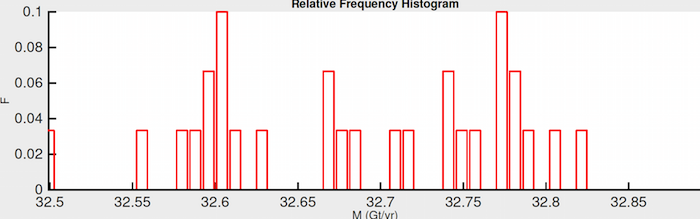
\includegraphics[width=\textwidth]{\assetsParentPath/assets/img/using-issm/tutorials/uncertaintyquantification/SamplingResults.png}
	\end{center}
\end{figure}

Plot Sensitivity Results:
\begin{itemize}
	\item To retrieve sensitivities for each model input:
		\begin{itemize}
			\item See lines 288-290
		\end{itemize}
	\item To plot sensitivities:
		\begin{itemize}
			\item See lines 292-300
		\end{itemize}

	\item To retrieve importance factors for each model input:
		\begin{itemize}
			\item See lines 303-305
		\end{itemize}
	\item To plot the importance factors:
		\begin{itemize}
			\item See lines 307-314
		\end{itemize}

	\item Run step 7, this step will result in two images. The first is the sensitivities (S), and the second in the importance factors (If, sensitivities scaled by input errors).
\end{itemize}
\begin{figure}[H]
	\begin{center}
		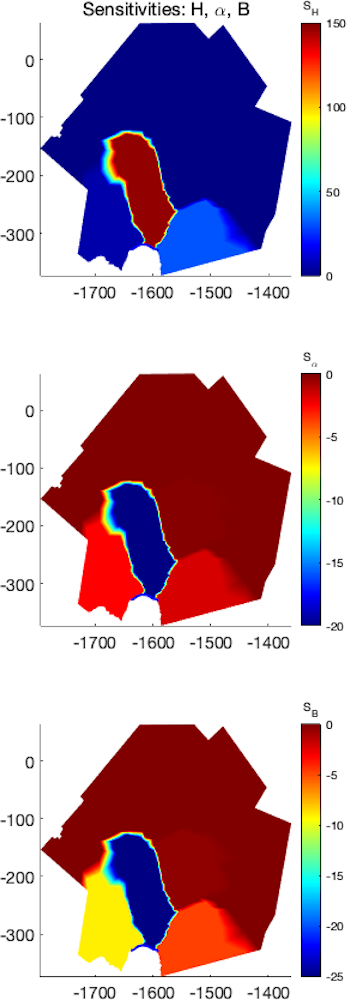
\includegraphics[width=0.475\textwidth]{\assetsParentPath/assets/img/using-issm/tutorials/uncertaintyquantification/PlotSensitivities.png}
		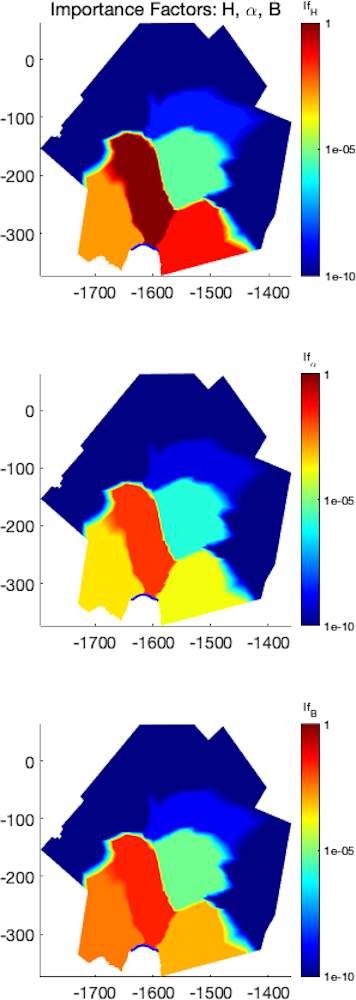
\includegraphics[width=0.475\textwidth]{\assetsParentPath/assets/img/using-issm/tutorials/uncertaintyquantification/ImportanceFactors.png}
	\end{center}
\end{figure}
%}}}
\subsubsection{Additional Exercises} %{{{
\begin{itemize}
	\item Add diagnostic IceVolume or MaxVelocity
	\item Sample with a uniform distribution (See \lstinlinebg|help uniform_uncertain|)
	\item Sample additional variables (i.e. friction coefficient, ice rheology)
	\item Try qmu on a different solution type
	\item Change number of partitions. Note: for sensitivity this could take a while!
\end{itemize}
%}}}

\clearpage % Make sure all figures are placed before next section
